\section{Considerações Iniciais}

A Arquitetura \textit{Speech2Learning} foi motivada por um MS prévio, detalhado na \autoref{section:foundation:sm}, cujo objetivo foi identificar o papel da tecnologia no ensino e aprendizagem, particularmente através das línguas de sinais \cite{FalvoJr2020_SBIE, FalvoJr2020_FIE, FalvoJr2021_RENOTE}. Este estudo proporcionou uma visão abrangente sobre o uso das TICs para o desenvolvimento de TA, evidenciando a importância significativa de novas tecnologias para um processo de ensino-aprendizagem mais inclusivo.

Contudo, foi observada uma lacuna importante: a ausência de padrões e boas práticas de desenvolvimento que facilitassem o compartilhamento e reuso de OAs. Como resposta a essa necessidade, a Arquitetura \textit{Speech2Learning} foi estabelecida para promover a criação de soluções estruturalmente preparadas para a inclusão, não apenas de pessoas surdas, mas também de aprendizes que necessitam de maior acessibilidade em conteúdos educacionais audíveis \cite{FalvoJr2023_HICSS}.

Além disso, a \textit{Speech2Learning} adota uma abordagem modular e escalável, permitindo que diferentes componentes de reconhecimento de fala e processamento de áudio sejam integrados de forma flexível. Isso possibilita que a arquitetura se adapte a diversos contextos educacionais e necessidades específicas dos aprendizes. A arquitetura também enfatiza a interoperabilidade e a conformidade com padrões abertos, facilitando a integração com outras plataformas e ferramentas educacionais, promovendo um ecossistema mais colaborativo e acessível.

A evolução da área de IA, especialmente com modelos generativos, tem o potencial de expandir ainda mais as capacidades da \textit{Speech2Learning}. A IAGen, com a habilidade de processar e gerar texto de forma autônoma, pode ser utilizada para aprimorar a acessibilidade e a personalização dos OAs, abrindo novas possibilidades para a criação de conteúdo e interação com os alunos.

Nesse sentido, a \textit{Speech2Learning} não apenas aborda a lacuna identificada em relação à falta de padrões, mas também estabelece um \textit{framework} robusto e inclusivo para o desenvolvimento de soluções educacionais baseadas em reconhecimento automático de fala. Esta arquitetura visa transformar a maneira como os conteúdos educacionais audíveis são criados e acessados, promovendo uma educação mais inclusiva e acessível para todos os aprendizes.

\section{Principais Referências e Inspirações}

Tecnicamente, a \textit{Speech2Learning} propõe um arcabouço genérico que vai além das línguas de sinais, escopo inicial do MS conduzido neste trabalho \cite{FalvoJr2020_SBIE, FalvoJr2020_FIE, FalvoJr2021_RENOTE}. No entanto, ele fornece uma abstração que facilita a acessibilidade de OAs audíveis, permitindo a geração de transcrições e, consequentemente, a sinalização do conteúdo educacional em questão. Nesse contexto, soluções baseadas em avatares, tais como \textit{Hand Talk} ou \textit{VLibras}, podem ser utilizadas com base nas transcrições, tornando os conteúdos acessíveis para usuários das línguas de sinais.

Sendo assim, foi proposta a Arquitetura \textit{Speech2Learning}, uma adaptação da \textit{Clean Architecture} de \citeonline{martin2017}, com o objetivo específico de promover a acessibilidade de OAs por meio do reconhecimento de fala. Segundo \citeonline{martin2017}, a \textit{Clean Architecture} é uma ideia prática que integra algumas das principais referências em ES nas últimas décadas \cite{cockburn2005, freeman2009, palermo2008, coplien2012, reenskaug2009, jacobson1992}. 

Essas iniciativas compartilham a ideia central de separar o código em camadas independentes, com o domínio no núcleo da arquitetura. Isso permite a criação de sistemas altamente testáveis, independentes de tecnologia, e adaptáveis às necessidades específicas de um projeto. A Arquitetura \textit{Speech2Learning}, alinhada a esses princípios, concentra seu domínio de aplicação central nos OAs, conforme representado pela \autoref{fig:chapter3-speech2learning-arch}. 

\begin{figure}[htb]
\centering
\caption{Arquitetura \textit{Speech2Learning}}
\label{fig:chapter3-speech2learning-arch}
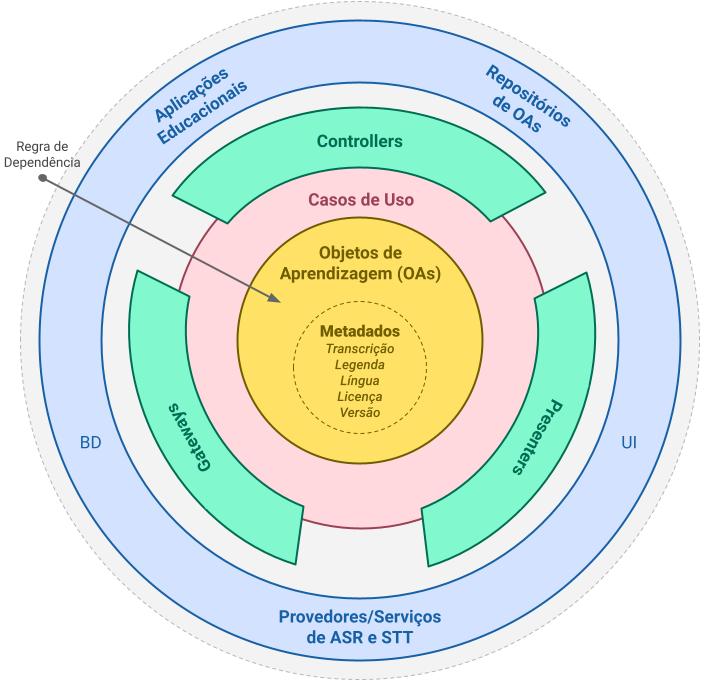
\includegraphics[width=0.71\textwidth]{images/chapter3-speech2learning-arch.png}
\fadaptada{FalvoJr2023_HICSS}
\end{figure}

Cada camada da \textit{Speech2Learning} contribui de forma significativa para OAs mais acessíveis por meio dos conceitos de ASR/STT, os quais, em conjunto com os metadados, são cruciais para promover a acessibilidade dos OAs de forma padronizada e consistente. Vale ressaltar que uma arquitetura não tem como objetivo definir detalhes de implementação, mas sim abstrações de software que podem ser adaptadas de acordo com as necessidades de cada domínio de aplicação. A seguir, apresenta-se uma síntese de cada uma das camadas definidas pela Arquitetura \textit{Speech2Learning}:

\begin{itemize}
\item \textbf{Objetos de Aprendizagem (Amarelo)}: Responsável pelos modelos e regras de negócio do domínio. Para garantir que os OAs sejam mais acessíveis e padronizados, as entidades podem incluir transcrição, legendagem e outras capacidades compatíveis com o domínio de aplicação e o padrão de metadados dos OAs audíveis. Além disso, o processo de reconhecimento de fala deve ser, idealmente, multimodal (abrangendo áudio e vídeo) e suportar múltiplos idiomas. Nesse sentido, considerar IAs, especialmente as generativas, é recomendado uma vez que elas resolvem de forma efetiva muitos desses desafios técnicos. Sendo assim, desde o centro da nossa arquitetura, onde estão os OAs, se faz necessária uma visão de projeto arquitetural que tenha sinergia com IAGen;
\item \textbf{Casos de Uso (Vermelho)}: Operações de alto nível e regras de negócio do sistema. Em outras palavras, esta camada é responsável por orquestrar as regras encapsuladas nos OAs, função comumente chamada de ``dança das entidades'';
\item \textbf{Adaptadores (Verde)}: Tem a responsabilidade de converter os dados para um formato conveniente, considerando as necessidades das camadas com as quais faz fronteira;
\item \textbf{Infraestrutura (Azul)}: Abrange questões técnicas e específicas, como \textit{frameworks}, \textit{drivers} e integrações externas. Nesse sentido, conexões com \sigla{BDs}{Bancos de Dados}, serviços de ASR/STT ou eventuais integrações com APIs de IAGen fariam parte desta camada. Além disso, ela inclui a \sigla{UI}{Interface do Usuário}, abrangendo a conexão com aplicações educacionais concretas (\textit{d-learning}, \textit{e-learning}, \textit{m-learning} etc) ou repositórios de OAs;
\item \textbf{Principal e Configuração (Cinza)}: Estabelece todas as conexões entre interfaces e suas implementações concretas, além de ser responsável por configurar e executar a aplicação.
\end{itemize}

A ``Regra de Dependência'' define que as dependências de código devem apontar apenas para dentro, em direção aos OAs, nunca para fora. Desse modo, a \textit{Speech2Learning} favorece a adaptabilidade, independência tecnológica e testabilidade, fornecendo uma orientação estrutural para a criação de soluções educacionais mais acessíveis. 

Portanto, é fundamental que as responsabilidades e boas práticas de suas camadas sejam bem compreendidas, pois elas estruturam diretrizes de projeto genéricas para a criação de soluções de TA baseadas em ASR. As seções a seguir detalham cada uma dessas camadas.

\section{Camada de Entidades (Objetos de Aprendizagem)}

\begin{figure}[htb]
\centering
\caption{Camada de Entidades (Objetos de Aprendizagem)}
\label{fig:chapter3-speech2learning-layer1}
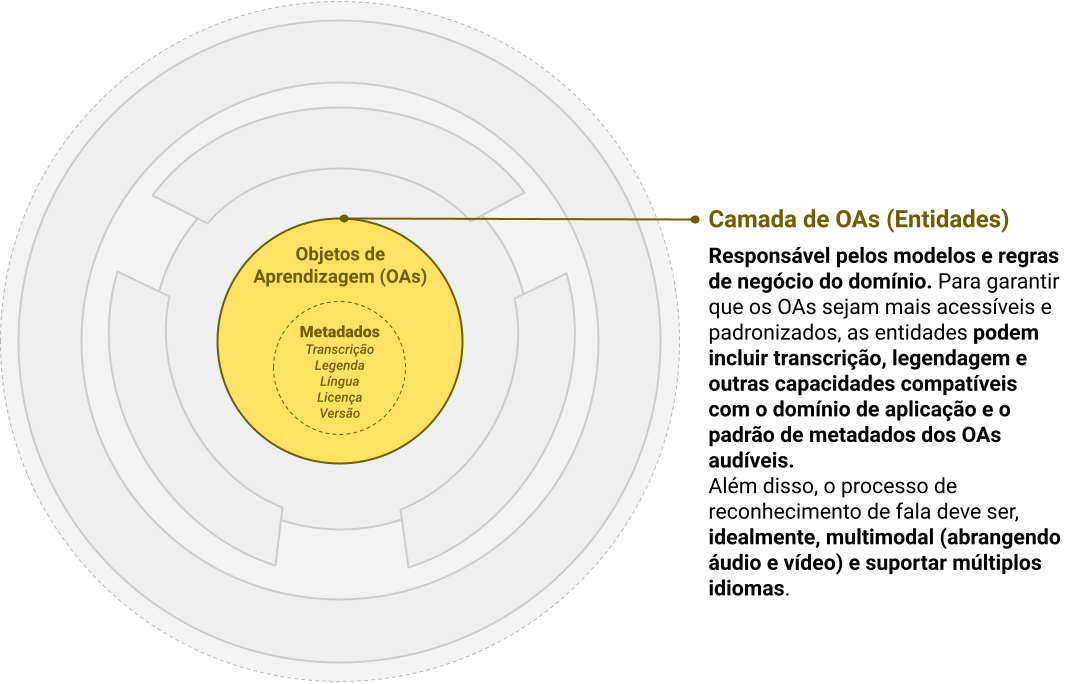
\includegraphics[width=1\textwidth]{images/chapter3-speech2learning-layer1.png}
\fadaptada{FalvoJr2023_HICSS,Lemos2022}
\end{figure}

A Camada de Entidades na Arquitetura \textit{Speech2Learning} é central para a definição dos modelos e regras de negócio do domínio dos OAs (\autoref{fig:chapter3-speech2learning-layer1}). Esta camada é responsável por encapsular os dados fundamentais e as lógicas que regem a estrutura e o comportamento dos OAs, garantindo sua acessibilidade e padronização. 

Para alcançar esses objetivos, é crucial incorporar padrões de metadados estabelecidos, como Dublin Core, SCORM, MISB, LOM e RDF, que fornecem diretrizes consistentes para a definição e organização dos conteúdos educacionais \cite{Santana2023}. As principais responsabilidades da Camada de Entidades incluem:

\begin{itemize}
    \item \textbf{Modelagem dos OAs}: Definir e estruturar os OAs de forma a garantir sua acessibilidade. Isso inclui a inclusão de elementos como transcrição, legendagem e outros recursos que tornam os conteúdos audíveis acessíveis a uma ampla gama de aprendizes, incluindo aqueles com necessidades especiais.

    \item \textbf{Definição de Regras de Negócio do Domínio}: Estabelecer regras de negócio que governam o comportamento dos OAs, assegurando que os processos de ensino-aprendizagem sejam eficazes e inclusivos. As regras de negócio devem considerar a multimodalidade do reconhecimento de fala, abrangendo áudio e vídeo, e suportando múltiplos idiomas.

    \item \textbf{Padronização e Interoperabilidade}: Garantir que os OAs sejam compatíveis com os padrões de metadados, facilitando seu compartilhamento e reuso em diferentes plataformas educacionais. A conformidade com padrões como Dublin Core, SCORM, MISB, LOM e RDF é essencial para manter a consistência e a qualidade dos OAs.
\end{itemize}

Os padrões de metadados desempenham um papel crucial na definição e organização dos OAs. A seguir, ilustra-se como cada padrão pode ser aplicado na Camada de OAs (Entidades):

\begin{itemize}
    \item \textbf{Dublin Core}: Fornece um conjunto simples e genérico de elementos para descrever recursos digitais. Na Camada de Entidades, Dublin Core pode ser utilizado para definir metadados básicos como título, autor, descrição, data, formato e identificador dos OAs, facilitando sua catalogação e recuperação.

    \item \textbf{SCORM}: É um padrão para LMS que facilita o reuso de conteúdos educacionais. Na \textit{Speech2Learning}, SCORM pode ser utilizado para definir a estrutura modular dos OAs, permitindo que cada unidade de aprendizagem seja facilmente reutilizada e integrada em diferentes cursos e plataformas.

    \item \textbf{MISB}: Embora mais comum em contextos de vídeo e imagem em movimento, MISB pode ser aplicado para garantir que os conteúdos audiovisuais dos OAs sejam padronizados e interoperáveis, especialmente em termos de metadados de vídeo e áudio.

    \item \textbf{LOM}: É um padrão específico para descrever OAs. Na Camada de Entidades, LOM pode ser utilizado para definir metadados detalhados que incluem, além dos elementos básicos, informações pedagógicas como tipo de recurso, nível de dificuldade, tempo de aprendizagem e público-alvo.

    \item \textbf{RDF}: Facilita a interoperabilidade de dados na web. Na \textit{Speech2Learning}, RDF pode ser utilizado para criar descrições estruturadas e semânticas dos OAs, permitindo que os dados sobre os objetos sejam facilmente compartilhados e integrados com outros sistemas e plataformas educacionais.
\end{itemize}

Do ponto de vista prático, o \autoref{codigo:exemplo-camada1} exemplifica o modelo \textit{TranscribedAudio}, o qual estabelece uma conexão com as responsabilidades citadas. Além disso, elementos fundamentais como documentação, convenções e boas práticas se mostram presentes. Outro aspecto fundamental é a independência de \textit{frameworks} e bibliotecas, caracterizando uma entidade limpa.

\begin{codigo}[caption={Exemplo Camada de Entidades: Disponível em \url{https://bit.ly/S2L-Entity}}, label={codigo:exemplo-camada1}, language=Java, breaklines=true]
/**
 * Model that represents an audio file and its transcript.
 * Responsibilities:
 * - Hold properties: ID, name, content, transcript.
 * - Validate integrity and conformity of audio data.
 * Adherence to Clean Architecture:
 * - Central to business logic and rules.
 * - Independent of frameworks or data persistence.
 * 
 * Author: @falvojr
 */
public class TranscribedAudio {
  private String id, name, transcript;
  private InputStream content;

  public void validate() {
    if (empty(name) || empty(transcript) || empty(content)) {
      String msg =  "Name, transcript and content required.";
      throw new EnterpriseBusinessException(msg);
    }
    String ext = FileUtils.getExtension(name).toLowerCase();
    if (!VALID_EXT.contains(ext)) {
      String msg =  "Invalid ext, use %s".formatted(VALID_EXT);
      throw new EnterpriseBusinessException(msg);
    }
  }
}
\end{codigo}

Por fim, para garantir maior acessibilidade e internacionalização dos OAs, é essencial que esta camada considere o ASR de forma multimodal, abrangendo tanto áudio quanto vídeo. Isso permite que os conteúdos educacionais audíveis sejam mais diversos e flexíveis às diferentes necessidades dos aprendizes. Além disso, a capacidade de suportar múltiplos idiomas é fundamental para a inclusão de aprendizes de diversas origens linguísticas, promovendo uma educação verdadeiramente inclusiva e global.

Adicionalmente, a IAGen pode ser utilizada para enriquecer os metadados dos OAs, gerando automaticamente descrições mais detalhadas e informativas, \textit{tags} relevantes e até mesmo traduções para diferentes idiomas, aumentando a descoberta e a reutilização dos OAs em diferentes contextos e por diferentes públicos.

\section{Camada de Aplicação (Casos de Uso)}

\begin{figure}[htb]
\centering
\caption{Camada de Aplicação (Casos de Uso)}
\label{fig:chapter3-speech2learning-layer2}
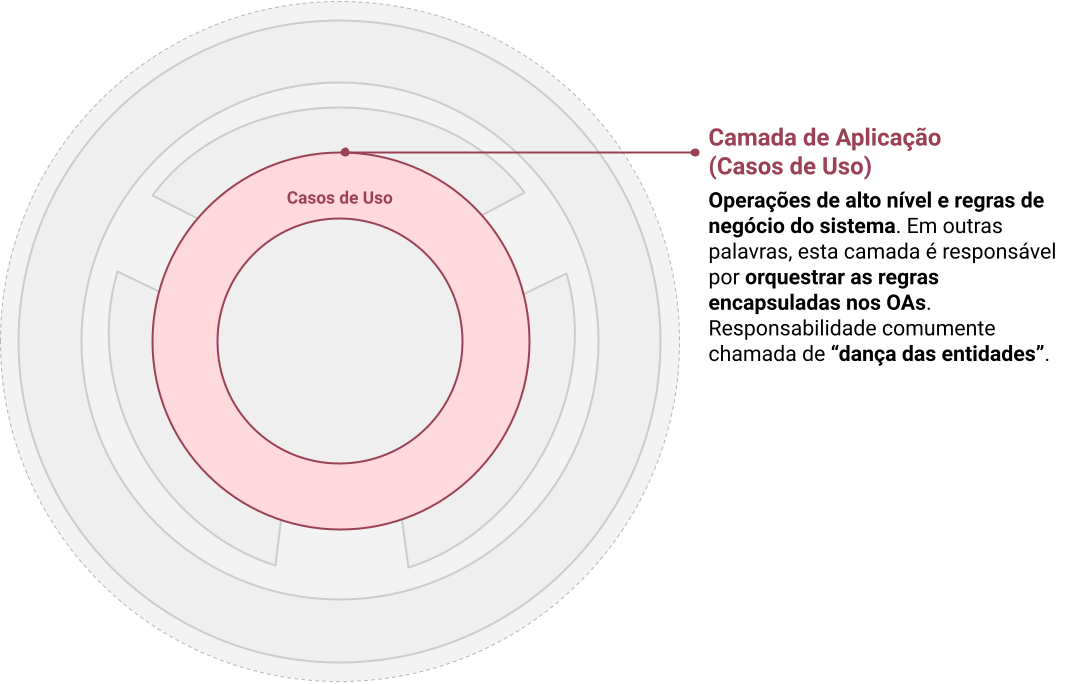
\includegraphics[width=.98\textwidth]{images/chapter3-speech2learning-layer2.png}
\fadaptada{FalvoJr2023_HICSS, Lemos2022}
\end{figure}

A Camada de Aplicação na arquitetura \textit{Speech2Learning} é responsável pela implementação das regras de negócio da aplicação, ou seja, dos casos de uso. Esta camada orquestra as operações de alto nível, garantindo que as regras encapsuladas nos OAs sejam executadas de maneira eficiente e coerente com os objetivos educacionais e de acessibilidade da arquitetura (\autoref{fig:chapter3-speech2learning-layer2}). As principais responsabilidades da Camada de Aplicação incluem:

\begin{itemize}
    \item \textbf{Orquestração de Regras de Negócio}: Implementar e gerenciar as regras de negócio que definem o comportamento dos OAs, garantindo que as operações de ensino e aprendizagem sejam conduzidas de maneira consistente com os objetivos de acessibilidade e inclusão.

    \item \textbf{Coordenação de Fluxos de Trabalho}: Coordenar os diversos fluxos de trabalho relacionados aos processos de ensino-aprendizagem, incluindo a transcrição, legendagem e geração de metadados, assegurando que todas as etapas sejam integradas de forma harmoniosa.

    \item \textbf{Interação com Outras Camadas}: Facilitar a comunicação entre a Camada de Entidades e as externas (Adaptadores e Infraestrutura), garantindo que as operações sejam executadas corretamente e que os dados sejam processados/transmitidos conforme necessário.
\end{itemize}

Na prática, algumas abstrações são essenciais para a implementação eficaz dos casos de uso. Como sugestões de abstrações que fazem sentido para essa arquitetura destacam-se:

\begin{itemize}
    \item \textbf{Controladores de Casos de Uso}: Classes ou componentes que implementam casos de uso específicos, orquestrando as operações de acordo com as regras de negócio. Por exemplo, um controlador pode gerenciar o processo de transcrição de um conteúdo de áudio, interagindo com a Camada de Entidades para armazenar os resultados e atualizar os metadados do OA.

    \item \textbf{Serviços de Aplicação}: Componentes que encapsulam lógica de negócio reutilizável, fornecendo funcionalidades comuns a múltiplos casos de uso. Exemplos incluem serviços para processamento de áudio, reconhecimento de fala ou geração de legendas, que podem ser utilizados por diferentes controladores de casos de uso.

    \item \textbf{Repositórios de Casos de Uso}: Interfaces e implementações que gerenciam a persistência e recuperação de dados necessários para a execução dos casos de uso. Estes repositórios abstraem o acesso aos dados, permitindo que a lógica de negócio permaneça desacoplada das questões de persistência.

    \item \textbf{\sigla{DTO}{\textit{Data Transfer Objects}}}: Objetos de transferência de dados utilizados para encapsular e transportar dados entre as diferentes camadas da arquitetura. Os DTOs garantem que os dados sejam transmitidos de maneira eficiente e coerente, facilitando a comunicação entre controladores de casos de uso e outros componentes do sistema.

    \item \textbf{Interfaces de Serviços Externos}: Abstrações que representam serviços externos necessários para a execução dos casos de uso, como APIs de ASR, serviços de tradução ou plataformas de gestão de conteúdos educacionais. Estas interfaces permitem que a Camada de Aplicação interaja com serviços externos de maneira flexível e desacoplada.
\end{itemize}

Nesse contexto, tem-se como exemplo um caso de uso que orquestra o processo de transcrição de áudio para texto, interagindo com serviços de reconhecimento de fala e atualizando os metadados do OA para incluir a transcrição gerada. Essa implementação fez parte de uma das POCs implementadas ao longo deste trabalho de doutorado e pode ser acessada neste repositório \textit{open-source}: \url{https://bit.ly/S2L-UseCase}.

Tais abstrações e exemplos demonstram como a Camada de Aplicação pode ser estruturada para orquestrar de forma eficiente os OAs aderentes aos princípios da \textit{Speech2Learning}, promovendo a acessibilidade por meio de soluções baseadas em reconhecimento de fala.

A IAGen pode também ser aplicada nesta camada para implementar casos de uso inovadores, como a geração automática de roteiros para videoaulas, a criação de \textit{chatbots} para interação com os aprendizes e a personalização do \textit{feedback} em atividades avaliativas.

\section{Camada de Adaptadores}

\begin{figure}[htb]
\centering
\caption{Camada de Adaptadores}
\label{fig:chapter3-speech2learning-layer3}
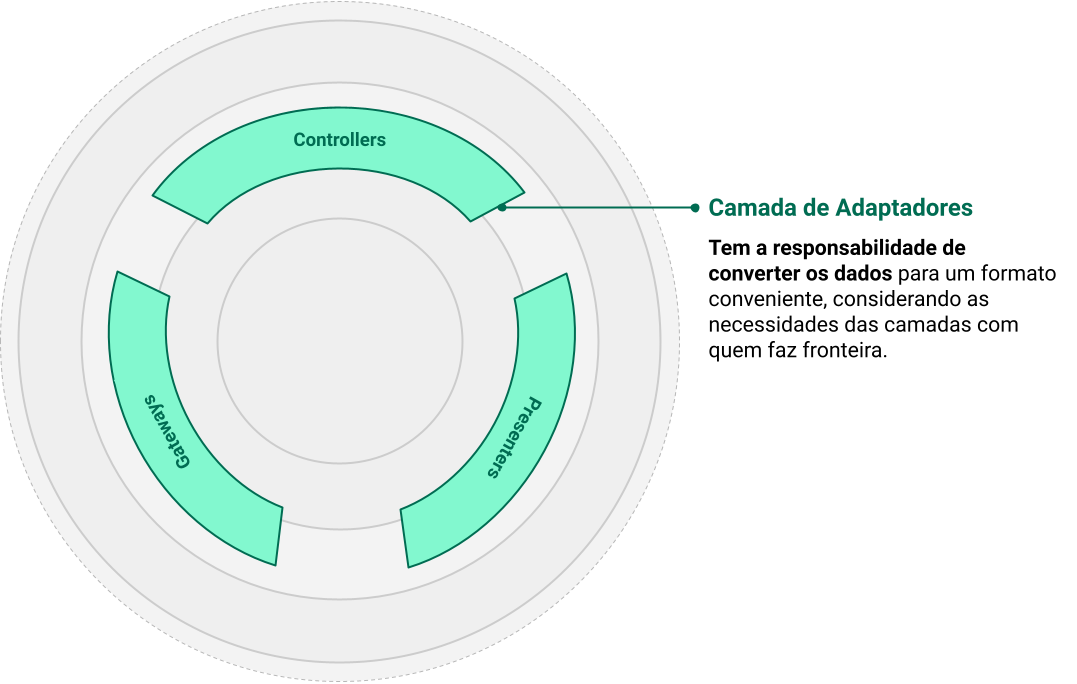
\includegraphics[width=.95\textwidth]{images/chapter3-speech2learning-layer3.png}
\fadaptada{FalvoJr2023_HICSS, Lemos2022}
\end{figure}

A Camada de Adaptadores na arquitetura \textit{Speech2Learning} tem a responsabilidade de converter os dados para um formato conveniente, considerando as necessidades das camadas com as quais faz fronteira. Esta camada atua como um intermediário crucial, garantindo que a comunicação entre as diferentes partes do sistema ocorra de maneira eficiente e coerente (\autoref{fig:chapter3-speech2learning-layer3}). As principais responsabilidades da Camada de Adaptadores incluem:

\begin{itemize}
    \item \textbf{Conversão de Dados}: Transformar os dados entre os formatos utilizados pelas camadas de Aplicação, Entidades e Infraestrutura, assegurando que cada camada receba os dados no formato mais adequado para sua funcionalidade.

    \item \textbf{Isolamento de Detalhes Técnicos}: Abstrair os detalhes técnicos de implementação, permitindo que as camadas superiores (Aplicação e Entidades) permaneçam independentes das preocupações técnicas específicas de integração com sistemas externos e infraestrutura.

    \item \textbf{Facilitação da Comunicação}: Garantir que a comunicação entre as diferentes camadas do sistema seja transparente e eficiente, minimizando os impactos de mudanças em uma camada sobre as demais.
\end{itemize}

Na \textit{Speech2Learning}, algumas abstrações são essenciais para a implementação eficaz dos adaptadores. Como sugestões de abstrações que fazem sentido para essa arquitetura destacam-se:

\begin{itemize}
    \item \textbf{Adaptadores de Entrada}: Componentes responsáveis por receber dados de fontes externas (como APIs, BDs ou UI) e convertê-los para um formato que possa ser processado pela Camada de Aplicação. Por exemplo, um adaptador de entrada pode receber dados de áudio de uma API de ASR e convertê-los em texto para processamento posterior.

    \item \textbf{Adaptadores de Saída}: Componentes que transformam dados gerados pela Camada de Aplicação em um formato que pode ser utilizado por sistemas externos ou armazenado em BDs. Por exemplo, um adaptador de saída pode transformar transcrições de texto em um formato adequado para armazenamento em um ROAs.

    \item \textbf{Interfaces de Conversão de Dados}: Abstrações que definem métodos para converter dados entre diferentes formatos e protocolos. Estas interfaces garantem que a lógica de conversão seja desacoplada das implementações específicas, promovendo reutilização e facilidade de manutenção.

    \item \textbf{Serviços de Mapeamento de Dados}: Componentes responsáveis por mapear diferentes estruturas de dados, simplificando a conversão de objetos complexos e a integração com sistemas variados. Por exemplo, um serviço pode converter objetos de uma linguagem de programação específica em metadados compatíveis com padrões como SCORM ou LOM.
\end{itemize}

Para ilustrar a aplicação das abstrações sugeridas, considere um exemplo de um adaptador de entrada que implementa um cliente HTTP, como o \textit{Open Feign}, para interagir com um serviço externo de transcrição, especificamente a API da OpenAI. Este adaptador recebe dados de áudio, converte-os para um formato adequado para a API, e traduz as respostas da API para um formato compreensível pelo domínio. 

Essa implementação foi desenvolvida em colaboração com a DIO e está disponível neste repositório \textit{open-source}: \url{https://bit.ly/S2L-Adapters}. Tais abstrações e exemplos demonstram como a Camada de Adaptadores pode ser estruturada para garantir a conversão eficiente de dados entre diferentes partes do sistema \textit{Speech2Learning}, promovendo a interoperabilidade e a flexibilidade necessárias para uma solução educacional baseada em reconhecimento de fala.

Adicionalmente, a IAGen pode ser integrada aos adaptadores para realizar tarefas como a tradução automática de legendas, a geração de descrições de áudio para pessoas com deficiência visual e a conversão de formatos de dados complexos em formatos mais simples e acessíveis.

\section{Camada de Infraestrutura}

\begin{figure}[htb]
\centering
\caption{Camada de Infraestrutura}
\label{fig:chapter3-speech2learning-layer4}
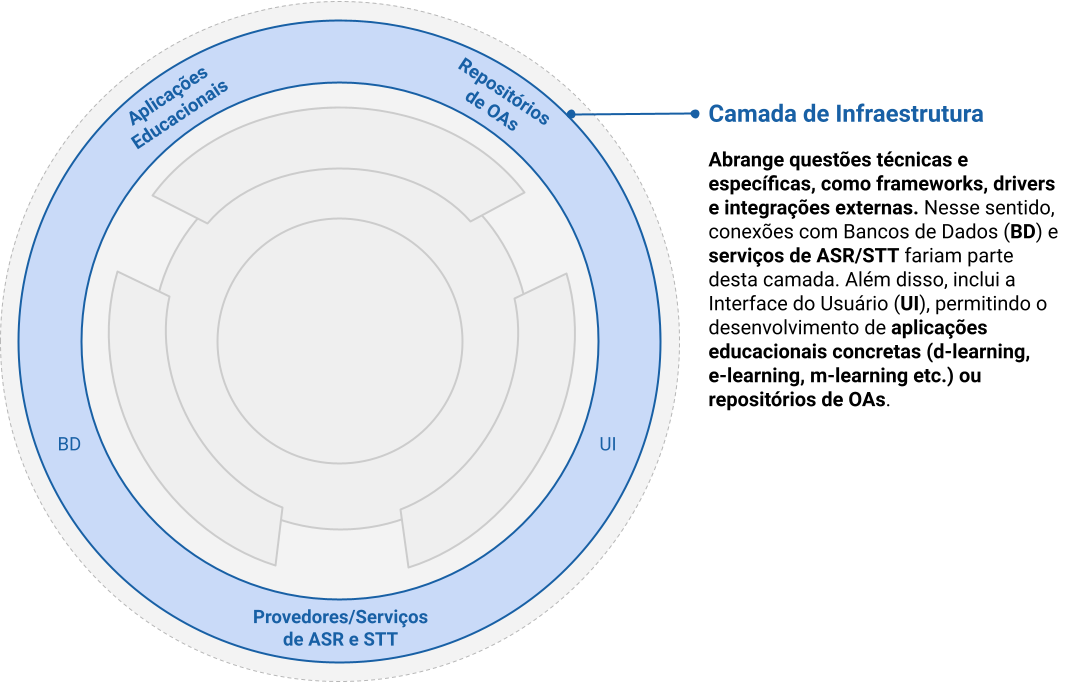
\includegraphics[width=1\textwidth]{images/chapter3-speech2learning-layer4.png}
\fadaptada{FalvoJr2023_HICSS, Lemos2022}
\end{figure}

A Camada de Infraestrutura na Arquitetura \textit{Speech2Learning} abrange questões técnicas e específicas, como \textit{frameworks}, \textit{drivers} e integrações externas. Nesse sentido, conexões com BDs e serviços de ASR/STT fazem parte desta camada. Além disso, inclui a Interface do Usuário (UI), permitindo o desenvolvimento de aplicações educacionais concretas (\textit{d-learning}, \textit{e-learning}, \textit{m-learning}, etc) ou repositórios de OAs (\autoref{fig:chapter3-speech2learning-layer4}). As principais responsabilidades da Camada de Infraestrutura incluem:

\begin{itemize}
    \item \textbf{Gerenciamento de Dados}: Conectar e interagir com sistemas de gerenciamento de BDs para armazenar, recuperar e manipular os dados necessários para a aplicação, garantindo que os dados sejam acessíveis e seguros.

    \item \textbf{Integrações Externas}: Gerenciar a comunicação com serviços externos, como APIs de reconhecimento de fala e serviços de tradução, garantindo que a aplicação possa utilizar funcionalidades fornecidas por terceiros.

    \item \textbf{Suporte a UI}: Fornecer a infraestrutura necessária para o desenvolvimento e operação das interfaces de usuário, permitindo que os aprendizes interajam com os OAs de maneira eficaz e intuitiva.

    \item \textbf{Manutenção de Infraestrutura Técnica}: Gerenciar componentes técnicos, incluindo \textit{drivers}, bibliotecas e \textit{frameworks}, que são essenciais para o funcionamento da aplicação, assegurando que todos os elementos estejam atualizados e funcionando corretamente.
\end{itemize}

Para a \textit{Speech2Learning}, algumas abstrações são essenciais para a implementação eficaz da infraestrutura. Entre as sugestões de abstrações que fazem sentido para essa arquitetura tem-se:

\begin{itemize}
    \item \textbf{Repositórios de Dados}: Interfaces e implementações responsáveis por gerenciar a persistência dos dados, encapsulando a lógica de acesso ao BD e garantindo a independência da Camada de Aplicação em relação às tecnologias de armazenamento.

    \item \textbf{Serviços de Integração}: Componentes que facilitam a comunicação com serviços externos, fornecendo interfaces padronizadas para interagir com APIs de reconhecimento de fala, serviços de tradução e outras ferramentas externas.

    \item \textbf{Gerenciadores de UI}: Abstrações que suportam o desenvolvimento e a operação das interfaces de usuário, assegurando que a experiência do usuário seja consistente e acessível.

    \item \textbf{\textit{Drivers} e Bibliotecas}: Componentes técnicos que fornecem funcionalidades específicas necessárias para a operação da aplicação, como \textit{drivers} de BDs, bibliotecas de manipulação de áudio e ferramentas de desenvolvimento de UI.
\end{itemize}

Para que se tenha uma perspectiva prática, segue um exemplo de um adaptador que implementa a persistência de dados de áudio transcritos utilizando o \textit{MongoDB} e seu sistema de arquivos \textit{GridFS}. Este adaptador lida com operações de \sigla{CRUD}{\textit{Create, Read, Update and Delete}} para entidades de áudio transcritas, gerenciando o armazenamento de conteúdo e metadados de maneira eficiente. Essa implementação está disponível no seguinte repositório \textit{open-source}: \url{https://bit.ly/S2L-Infra}.

Essas abstrações e exemplos demonstram como a Camada de Infraestrutura pode ser estruturada para fornecer o suporte técnico necessário para a Arquitetura \textit{Speech2Learning}, garantindo a interoperabilidade e a eficiência das operações de armazenamento e integração com serviços externos. Além disso, a IAGen pode ser utilizada para otimizar o desempenho da infraestrutura, por meio da análise de dados de uso e da identificação de padrões que permitam a alocação eficiente de recursos e a melhoria da escalabilidade do sistema.

\section{Pseudo-camada ``Principal \& Configuração''}

\begin{figure}[htb]
\centering
\caption{Pseudo-camada Principal \& Configuração}
\label{fig:chapter3-speech2learning-layer5}
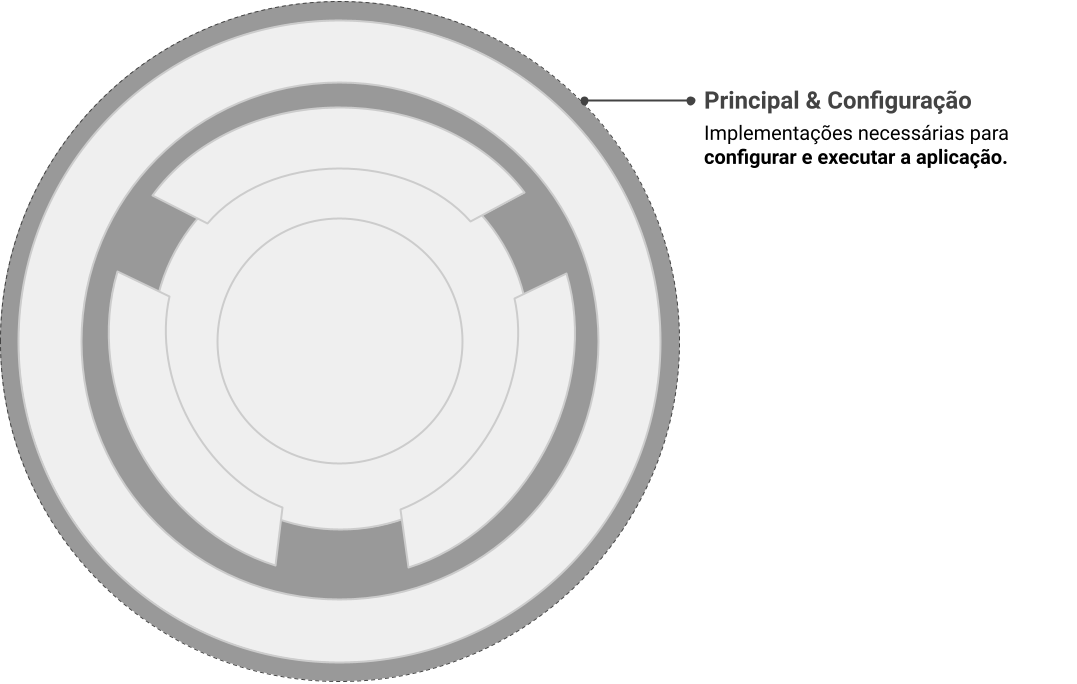
\includegraphics[width=1\textwidth]{images/chapter3-speech2learning-layer5.png}
\fadaptada{FalvoJr2023_HICSS, Lemos2022}
\end{figure}

A Pseudo-camada Principal \& Configuração na Arquitetura \textit{Speech2Learning} é assim denominada porque, embora não seja uma camada formal na \textit{Clean Architecture}, desempenha um papel crucial na configuração e inicialização do sistema. Em linhas gerais, esta camada estabelece todas as conexões entre interfaces e suas implementações concretas, além de ser responsável por configurar e executar a aplicação (\autoref{fig:chapter3-speech2learning-layer5}). Além disso, a camada centraliza a configuração e a inicialização, assegurando que todos os componentes estejam devidamente conectados e preparados para operar. As principais responsabilidades desta pseudo-camada incluem:

\begin{itemize}
    \item \textbf{Dependências}: Definir e gerenciar as dependências entre os diferentes componentes do sistema, garantindo que cada componente receba suas dependências de maneira clara e organizada. Isso promove a modularidade e facilita a manutenção do sistema.

    \item \textbf{Inicialização da Aplicação}: Coordenar o processo de inicialização da aplicação, assegurando que todos os componentes sejam configurados e instanciados na ordem correta. Isso inclui a configuração de serviços, repositórios, adaptadores e outros componentes essenciais.

    \item \textbf{Gerenciamento de Ciclo de Vida}: Controlar o ciclo de vida dos componentes, incluindo a criação, a configuração e a destruição de instâncias conforme necessário. Isso assegura que os recursos sejam gerenciados de maneira eficiente e que os componentes estejam sempre em um estado consistente.
\end{itemize}

Alguns exemplos de abstrações alinhadas à \textit{Speech2Learning} para a implementação da Pseudo-camada Principal \& Configuração, são:

\begin{itemize}
    \item \textbf{Módulos de Configuração}: Componentes que centralizam a configuração dos diferentes aspectos da aplicação, como casos de uso, repositórios de dados e serviços de integração. Estes módulos garantem que a configuração seja organizada e fácil de gerenciar.

    \item \textbf{Fábricas de Instâncias}: Abstrações que fornecem métodos para criar e configurar instâncias dos componentes do sistema. As fábricas asseguram que a criação de componentes siga um padrão consistente e que todas as dependências sejam satisfeitas.

    \item \textbf{Controladores de Inicialização}: Componentes responsáveis por coordenar o processo de inicialização da aplicação, garantindo que todos os componentes sejam configurados e preparados para operar. Os controladores de inicialização gerenciam a ordem de inicialização e tratam quaisquer dependências entre os componentes.
\end{itemize}

Para ilustrar a aplicação das abstrações listadas, considere um módulo de configuração que define e gerencia os casos de uso relacionados à transcrição de áudio. Este módulo centraliza a configuração das dependências necessárias para os casos de uso, promovendo a independência e a modularidade dos componentes em relação ao \textit{Spring Framework}. Exemplo em um projeto real disponível no repositório \textit{open-source}: \url{https://bit.ly/S2L-Adapters}.

Estas abstrações e exemplos demonstram como a Pseudo-camada Principal \& Configuração pode ser estruturada. Ao centralizar a configuração e a gestão de dependências, esta camada promove a modularidade e a flexibilidade necessárias para uma solução educacional baseada em reconhecimento de fala.

\section{Considerações Finais}

A Arquitetura \textit{Speech2Learning} foi concebida para promover a inclusão e a acessibilidade no domínio educacional, utilizando tecnologias avançadas de reconhecimento de fala, como o ASR e STT. Ao longo deste trabalho de doutorado, foi discutida a estrutura e as camadas fundamentais da \textit{Speech2Learning}, enfatizando sua modularidade, escalabilidade e conformidade com padrões de mercado. Essas características permitem que a arquitetura seja adaptável a diversos contextos educacionais e atenda às necessidades específicas de diferentes aprendizes, promovendo um ambiente de aprendizagem mais inclusivo e acessível.

A implementação das camadas da \textit{Speech2Learning} demonstrou como a integração de serviços de ASR e STT pode ser realizada de maneira estruturada e eficaz. A arquitetura não só facilita o desenvolvimento de soluções educacionais inclusivas, mas também promove a interoperabilidade entre diferentes plataformas e ferramentas educacionais. Além disso, a adoção de padrões de metadados como Dublin Core, SCORM, MISB, LOM e RDF garante que os OAs sejam estruturados de forma consistente e reutilizável, facilitando o compartilhamento de recursos educacionais.

A sinergia do conceito de IAGen na Arquitetura \textit{Speech2Learning} representa um avanço significativo na busca por soluções educacionais mais inclusivas, personalizadas e eficazes. Ao combinar o poder do ASR/STT com a capacidade de processamento de linguagem natural dos LLMs, a \textit{Speech2Learning} torna-se uma ferramenta poderosa para a criação e o acesso a OAs de alta qualidade, que atendem às necessidades de uma ampla gama de aprendizes.

É importante ressaltar que a adoção de IAGen na \textit{Speech2Learning} não é obrigatória, mas sim uma possibilidade que pode ser explorada para aprimorar ainda mais a arquitetura e suas funcionalidades. A flexibilidade da arquitetura permite que diferentes tecnologias e abordagens sejam integradas de acordo com as necessidades e os recursos disponíveis, garantindo que a \textit{Speech2Learning} continue a evoluir e a se adaptar às demandas do cenário educacional em constante transformação.

No próximo capítulo são apresentados os estudos de caso que ilustram a aplicação prática da \textit{Speech2Learning}. O primeiro estudo de caso avalia uma API para a transcrição e legendagem automática de videoaulas, integrando serviços de ASR de fornecedores líderes do mercado. O segundo estudo de caso explora o desenvolvimento de um player de vídeo com integração de avatares de Libras, destacando a importância do design universal para a inclusão de aprendizes surdos. Essas instâncias práticas da \textit{Speech2Learning} não só demonstram a versatilidade e a eficácia da arquitetura, mas também fornecem percepções valiosas sobre a implementação e a avaliação de soluções educacionais baseadas em reconhecimento de fala.